
%% bare_conf.tex
%% V1.4b
%% 2015/08/26
%% by Michael Shell
%% See:
%% http://www.michaelshell.org/
%% for current contact information.
%%
%% This is a skeleton file demonstrating the use of IEEEtran.cls
%% (requires IEEEtran.cls version 1.8b or later) with an IEEE
%% conference paper.
%%
%% Support sites:
%% http://www.michaelshell.org/tex/ieeetran/
%% http://www.ctan.org/pkg/ieeetran
%% and
%% http://www.ieee.org/

%%*************************************************************************
%% Legal Notice:
%% This code is offered as-is without any warranty either expressed or
%% implied; without even the implied warranty of MERCHANTABILITY or
%% FITNESS FOR A PARTICULAR PURPOSE! 
%% User assumes all risk.
%% In no event shall the IEEE or any contributor to this code be liable for
%% any damages or losses, including, but not limited to, incidental,
%% consequential, or any other damages, resulting from the use or misuse
%% of any information contained here.
%%
%% All comments are the opinions of their respective authors and are not
%% necessarily endorsed by the IEEE.
%%
%% This work is distributed under the LaTeX Project Public License (LPPL)
%% ( http://www.latex-project.org/ ) version 1.3, and may be freely used,
%% distributed and modified. A copy of the LPPL, version 1.3, is included
%% in the base LaTeX documentation of all distributions of LaTeX released
%% 2003/12/01 or later.
%% Retain all contribution notices and credits.
%% ** Modified files should be clearly indicated as such, including  **
%% ** renaming them and changing author support contact information. **
%%*************************************************************************


% *** Authors should verify (and, if needed, correct) their LaTeX system  ***
% *** with the testflow diagnostic prior to trusting their LaTeX platform ***
% *** with production work. The IEEE's font choices and paper sizes can   ***
% *** trigger bugs that do not appear when using other class files.       ***                          ***
% The testflow support page is at:
% http://www.michaelshell.org/tex/testflow/



\documentclass[10pt,conference]{IEEEtran}
% Some Computer Society conferences also require the compsoc mode option,
% but others use the standard conference format.
%
% If IEEEtran.cls has not been installed into the LaTeX system files,
% manually specify the path to it like:
% \documentclass[conference]{../sty/IEEEtran}





% Some very useful LaTeX packages include:
% (uncomment the ones you want to load)


% *** MISC UTILITY PACKAGES ***
%
%\usepackage{ifpdf}
% Heiko Oberdiek's ifpdf.sty is very useful if you need conditional
% compilation based on whether the output is pdf or dvi.
% usage:
% \ifpdf
%   % pdf code
% \else
%   % dvi code
% \fi
% The latest version of ifpdf.sty can be obtained from:
% http://www.ctan.org/pkg/ifpdf
% Also, note that IEEEtran.cls V1.7 and later provides a builtin
% \ifCLASSINFOpdf conditional that works the same way.
% When switching from latex to pdflatex and vice-versa, the compiler may
% have to be run twice to clear warning/error messages.






% *** CITATION PACKAGES ***
%
%\usepackage\cite
% cite.sty was written by Donald Arseneau
% V1.6 and later of IEEEtran pre-defines the format of the cite.sty package
% \cite{} output to follow that of the IEEE. Loading the cite package will
% result in citation numbers being automatically sorted and properly
% "compressed/ranged". e.g., [1], [9], [2], [7], [5], [6] without using
% cite.sty will become [1], [2], [5]--[7], [9] using cite.sty. cite.sty's
% \cite will automatically add leading space, if needed. Use cite.sty's
% noadjust option (cite.sty V3.8 and later) if you want to turn this off
% such as if a citation ever needs to be enclosed in parenthesis.
% cite.sty is already installed on most LaTeX systems. Be sure and use
% version 5.0 (2009-03-20) and later if using hyperref.sty.
% The latest version can be obtained at:
% http://www.ctan.org/pkg/cite
% The documentation is contained in the cite.sty file itself.






% *** GRAPHICS RELATED PACKAGES ***
%
\ifCLASSINFOpdf
   \usepackage[pdftex]{graphicx}
  % declare the path(s) where your graphic files are
  % \graphicspath{{../pdf/}{../jpeg/}}
  % and their extensions so you won't have to specify these with
  % every instance of \includegraphics
  % \DeclareGraphicsExtensions{.pdf,.jpeg,.png}
\else
  % or other class option (dvipsone, dvipdf, if not using dvips). graphicx
  % will default to the driver specified in the system graphics.cfg if no
  % driver is specified.
   \usepackage[dvips]{graphicx}
  % declare the path(s) where your graphic files are
  % \graphicspath{{../eps/}}
  % and their extensions so you won't have to specify these with
  % every instance of \includegraphics
  % \DeclareGraphicsExtensions{.eps}
\fi
% graphicx was written by David Carlisle and Sebastian Rahtz. It is
% required if you want graphics, photos, etc. graphicx.sty is already
% installed on most LaTeX systems. The latest version and documentation
% can be obtained at: 
% http://www.ctan.org/pkg/graphicx
% Another good source of documentation is "Using Imported Graphics in
% LaTeX2e" by Keith Reckdahl which can be found at:
% http://www.ctan.org/pkg/epslatex
%
% latex, and pdflatex in dvi mode, support graphics in encapsulated
% postscript (.eps) format. pdflatex in pdf mode supports graphics
% in .pdf, .jpeg, .png and .mps (metapost) formats. Users should ensure
% that all non-photo figures use a vector format (.eps, .pdf, .mps) and
% not a bitmapped formats (.jpeg, .png). The IEEE frowns on bitmapped formats
% which can result in "jaggedy"/blurry rendering of lines and letters as
% well as large increases in file sizes.
%
% You can find documentation about the pdfTeX application at:
% http://www.tug.org/applications/pdftex





% *** MATH PACKAGES ***
%
\usepackage{amsmath}
\usepackage{amssymb}
\usepackage{marvosym}
% A popular package from the American Mathematical Society that provides
% many useful and powerful commands for dealing with mathematics.
%
% Note that the amsmath package sets \interdisplaylinepenalty to 10000
% thus preventing page breaks from occurring within multiline equations. Use:
%\interdisplaylinepenalty=2500
% after loading amsmath to restore such page breaks as IEEEtran.cls normally
% does. amsmath.sty is already installed on most LaTeX systems. The latest
% version and documentation can be obtained at:
% http://www.ctan.org/pkg/amsmath





% *** SPECIALIZED LIST PACKAGES ***
%
%\usepackage{algorithmic}
% algorithmic.sty was written by Peter Williams and Rogerio Brito.
% This package provides an algorithmic environment fo describing algorithms.
% You can use the algorithmic environment in-text or within a figure
% environment to provide for a floating algorithm. Do NOT use the algorithm
% floating environment provided by algorithm.sty (by the same authors) or
% algorithm2e.sty (by Christophe Fiorio) as the IEEE does not use dedicated
% algorithm float types and packages that provide these will not provide
% correct IEEE style captions. The latest version and documentation of
% algorithmic.sty can be obtained at:
% http://www.ctan.org/pkg/algorithms
% Also of interest may be the (relatively newer and more customizable)
% algorithmicx.sty package by Szasz Janos:
% http://www.ctan.org/pkg/algorithmicx




% *** ALIGNMENT PACKAGES ***
%
%\usepackage{array}
% Frank Mittelbach's and David Carlisle's array.sty patches and improves
% the standard LaTeX2e array and tabular environments to provide better
% appearance and additional user controls. As the default LaTeX2e table
% generation code is lacking to the point of almost being broken with
% respect to the quality of the end results, all users are strongly
% advised to use an enhanced (at the very least that provided by array.sty)
% set of table tools. array.sty is already installed on most systems. The
% latest version and documentation can be obtained at:
% http://www.ctan.org/pkg/array


% IEEEtran contains the IEEEeqnarray family of commands that can be used to
% generate multiline equations as well as matrices, tables, etc., of high
% quality.




% *** SUBFIGURE PACKAGES ***
\ifCLASSOPTIONcompsoc
  \usepackage[caption=false,font=normalsize,labelfont=sf,textfont=sf]{subfig}
\else
  \usepackage[caption=false,font=footnotesize]{subfig}
\fi
% subfig.sty, written by Steven Douglas Cochran, is the modern replacement
% for subfigure.sty, the latter of which is no longer maintained and is
% incompatible with some LaTeX packages including fixltx2e. However,
% subfig.sty requires and automatically loads Axel Sommerfeldt's caption.sty
% which will override IEEEtran.cls' handling of captions and this will result
% in non-IEEE style figure/table captions. To prevent this problem, be sure
% and invoke subfig.sty's "caption=false" package option (available since
% subfig.sty version 1.3, 2005/06/28) as this is will preserve IEEEtran.cls
% handling of captions.
% Note that the Computer Society format requires a larger sans serif font
% than the serif footnote size font used in traditional IEEE formatting
% and thus the need to invoke different subfig.sty package options depending
% on whether compsoc mode has been enabled.
%
% The latest version and documentation of subfig.sty can be obtained at:
% http://www.ctan.org/pkg/subfig




% *** FLOAT PACKAGES ***
%
%\usepackage{fixltx2e}
% fixltx2e, the successor to the earlier fix2col.sty, was written by
% Frank Mittelbach and David Carlisle. This package corrects a few problems
% in the LaTeX2e kernel, the most notable of which is that in current
% LaTeX2e releases, the ordering of single and double column floats is not
% guaranteed to be preserved. Thus, an unpatched LaTeX2e can allow a
% single column figure to be placed prior to an earlier double column
% figure.
% Be aware that LaTeX2e kernels dated 2015 and later have fixltx2e.sty's
% corrections already built into the system in which case a warning will
% be issued if an attempt is made to load fixltx2e.sty as it is no longer
% needed.
% The latest version and documentation can be found at:
% http://www.ctan.org/pkg/fixltx2e


\usepackage{stfloats}
% stfloats.sty was written by Sigitas Tolusis. This package gives LaTeX2e
% the ability to do double column floats at the bottom of the page as well
% as the top. (e.g., "\begin{figure*}[!b]" is not normally possible in
% LaTeX2e). It also provides a command:
%\fnbelowfloat
% to enable the placement of footnotes below bottom floats (the standard
% LaTeX2e kernel puts them above bottom floats). This is an invasive package
% which rewrites many portions of the LaTeX2e float routines. It may not work
% with other packages that modify the LaTeX2e float routines. The latest
% version and documentation can be obtained at:
% http://www.ctan.org/pkg/stfloats
% Do not use the stfloats baselinefloat ability as the IEEE does not allow
% \baselineskip to stretch. Authors submitting work to the IEEE should note
% that the IEEE rarely uses double column equations and that authors should try
% to avoid such use. Do not be tempted to use the cuted.sty or midfloat.sty
% packages (also by Sigitas Tolusis) as the IEEE does not format its papers in
% such ways.
% Do not attempt to use stfloats with fixltx2e as they are incompatible.
% Instead, use Morten Hogholm'a dblfloatfix which combines the features
% of both fixltx2e and stfloats:
%
% \usepackage{dblfloatfix}
% The latest version can be found at:
% http://www.ctan.org/pkg/dblfloatfix




% *** PDF, URL AND HYPERLINK PACKAGES ***
%
%\usepackage{url}
% url.sty was written by Donald Arseneau. It provides better support for
% handling and breaking URLs. url.sty is already installed on most LaTeX
% systems. The latest version and documentation can be obtained at:
% http://www.ctan.org/pkg/url
% Basically, \url{my_url_here}.




% *** Do not adjust lengths that control margins, column widths, etc. ***
% *** Do not use packages that alter fonts (such as pslatex).         ***
% There should be no need to do such things with IEEEtran.cls V1.6 and later.
% (Unless specifically asked to do so by the journal or conference you plan
% to submit to, of course. )


% correct bad hyphenation here
\hyphenation{op-tical net-works semi-conduc-tor}

%% Aiporre and Oamestegui : Commands 
\newcommand{\marco}[1]{\{\mathcal{#1}\}}
\begin{document}
%
% paper title
% Titles are generally capitalized except for words such as a, an, and, as,
% at, but, by, for, in, nor, of, on, or, the, to and up, which are usually
% not capitalized unless they are the first or last word of the title.
% Linebreaks \\ can be used within to get better formatting as desired.
% Do not put math or special symbols in the title.
\title{ Rotation Matrix Reconstruction in Quaternions with an Optimal Observer within a Navigation Algorithm Based on Nonlinear Complementary Observers }

% author names and affiliations
% use a multiple column layout for up to three different
% affiliations
%\author{\IEEEauthorblockN{Ariel Iporre}
%\IEEEauthorblockA{Enginering Faculty\\Electronic Engineering\\
%Universidad Mayor de San Andr\'es\\
%La Paz, Bolivia\\
%Email: aiporre@umsa.bo}
%\and
%\IEEEauthorblockN{Mauricio Am\'estegui}
%\IEEEauthorblockA{Enginering Faculty\\Electronic Engineering\\
%Universidad Mayor de San Andr\'es\\
%La Paz, Bolivia\\
%Email: mauricioamestegui@gmail.com}
%}
\author{\IEEEauthorblockN{Ariel Iporre Rivas\IEEEauthorrefmark{1} and
Mauricio Am\'estegui Moreno\IEEEauthorrefmark{2}}
\IEEEauthorblockA{\IEEEauthorrefmark{1}\IEEEauthorrefmark{2}Electronic Engineering - Engineering Department\\Universidad Mayor de San Andr\'es,
La Paz, Bolivia\\ Email: \IEEEauthorrefmark{1}aiporre@umsa.bo, \IEEEauthorrefmark{2}mauricioamestegui@gmail.com}}
% conference papers do not typically use \thanks and this command
% is locked out in conference mode. If really needed, such as for
% the acknowledgment of grants, issue a \IEEEoverridecommandlockouts
% after \documentclass

% for over three affiliations, or if they all won't fit within the width
% of the page, use this alternative format:
% 
%\author{\IEEEauthorblockN{Michael Shell\IEEEauthorrefmark{1},
%Homer Simpson\IEEEauthorrefmark{2},
%James Kirk\IEEEauthorrefmark{3}, 
%Montgomery Scott\IEEEauthorrefmark{3} and
%Eldon Tyrell\IEEEauthorrefmark{4}}
%\IEEEauthorblockA{\IEEEauthorrefmark{1}School of Electrical and Computer Engineering\\
%Georgia Institute of Technology,
%Atlanta, Georgia 30332--0250\\ Email: see http://www.michaelshell.org/contact.html}
%\IEEEauthorblockA{\IEEEauthorrefmark{2}Twentieth Century Fox, Springfield, USA\\
%Email: homer@thesimpsons.com}
%\IEEEauthorblockA{\IEEEauthorrefmark{3}Starfleet Academy, San Francisco, California 96678-2391\\
%Telephone: (800) 555--1212, Fax: (888) 555--1212}
%\IEEEauthorblockA{\IEEEauthorrefmark{4}Tyrell Inc., 123 Replicant Street, Los Angeles, California 90210--4321}}




% use for special paper notices
%\IEEEspecialpapernotice{(Invited Paper)}




% make the title area
\maketitle

% As a general rule, do not put math, special symbols or citations
% in the abstract
\begin{abstract}
This work proposes a variation for a earlier navigation algorithm in the literature composed by SO(3) complementary observers. Such modification involves the inclusion of a quaternion optimal observer to determine  the rotation matrix instead using a vectorial reconstruction approach, in particular this proposal involves an experimental comparison between the original and modified method. The results show about 40\% increase for estimation quality while 21\% more complexity using this new approach. 
\end{abstract}

% no keywords




% For peer review papers, you can put extra information on the cover
% page as needed:
% \ifCLASSOPTIONpeerreview
% \begin{center} \bfseries EDICS Category: 3-BBND \end{center}
% \fi
%
% For peerreview papers, this IEEEtran command inserts a page break and
% creates the second title. It will be ignored for other modes.
\IEEEpeerreviewmaketitle
\section{Introduction}
Roughly speaking the process of moving between two points implies determine the position and direction throughout all the trajectory. This problem is generally solved by interpreting measurements from fixed references or variables revealing the internal states of the motion body. Hereby, navigation can defined as the art of calculate or interpret this variables and the set elements inferring such results are  known as Navigation System. Furthermore, a navigation system incorporates a navigation algorithm that tweaks the motion models optimizing the predictions much like the way of a control systems.  In fact, the famous Kalman Optimal Observer solving the Winner-Hoft optimal observer problem presents itself as a consequence of the duality control-observer principle \cite{Kalman1960}, thus the author extends a spectral statistical filter to make predictions in time recalling principles from the Optimal Control Theory. Moreover, most recent trends for designing this kind of observers also explode tools from control theory that is nonlinear filters developed in the framework of Lyapunov theory e.g. \cite{Lukyanov1996,Nicosia1996}. Further, some authors worked to reduce the complexity involved in navigation equations by dividing the process in separated observers, for example in \cite{Vasconcelos2008} two observers are combined first to determine the rotation matrix and then to calculate the position, or in \cite{Scandaro2011} who combine to complementary filters to determine rotation and position in two separated processes.  Therefore, based on this initial idea, in this work we propose the calculation of the rotational matrix in quaternions using an optimal observer by modifying the initial navigation algorithm proposed in \cite{Scandaro2011}.\par
%
One of the first formal approaches dealing the navigation problem was addressed as an application of the famous Kalman Filter which has been extended through the linear perturbation equation to solve the trajectory estimation for a nonlinear model of motion and its was used to unravel the trajectory from motion signals in navigation computer of the Apollo project \cite{Schmidt1962}.  In the Kalman Filter's original paper, the authors re-casted the optimal estimation methods developed by Norbert Wiener (Stationary Stochastic Signals) in terms of first and second momentum matrices of conditional probabilities in the states space form which allots the same solution to non-stationaty signals embedded in the discrete time version of the Riccati equation \cite{Grewal2010}. Since that milestone event many other authors have issued an enormous quantity of ideas diverging from Kalman's core paper in the field of navigation algorithms e.g. \cite{Bistrovs2012, Gandhi2007}. Some versions of the Kalman Filter work with powerful representation of motion based on atypical algebraic structures like quaternions, \cite{Marins2001} pre-calculates the quaternion using a Gauss-Newton iteration algorithm to find the best quaternion that relates the measured accelerations and earth magnetic field in the body coordinate frame, they addressed with a similar approach to what is followed in this work in the sense that we pre-compute the rotation matrix as they did.\par 
%
There exists a high cohesion between the ideas of design of Luenberger Observers and the optimal approach followed by the Kalman Filter, in deed the target of the Luenberger Observer is to determine unknown states as in the Kalman Filter with the difference of that Luenberger works within dynamical system framework  and avoids to use statistical terminology \cite{Luenberger1966}. Luenberger develops theoretical foundation through the use of modern control applied to the observer problem, which triggers the engagement of non-linear control theory e.g. \cite{Kou1975}\cite{Thau1973} in this field. Further trends in this approach work to implement non linear observers when the system's dynamic entails impossible linearize nonlinear terms as the navigation equations, hence this approach has been used to develop navigation algorithms founded in  the design of Lyapunov and exponential stability, and again they grip to strong rugged representation of rotation using quaternions \cite{Vik2001} \cite{Thienel2003} and \cite{Hua2009}. Quaternion algebra plays a mayor role in nonlinear observers simplifying calculations and offering good algebraic structure that allows to recover angles without singularities.\par
%%
Further, an special approach is extended by \cite{Bonabel2008} which proposes a general geometrical framework for the design of observers on finite-dimensional Lie groups. One particular case investigated in \cite{Bonabel2008} explains the general form of non-linear observers on SO(3) where the dynamics and the correction terms are expressed on a tangential Lie Algebras $\mathfrak{so}(3)$, further the orientation is determined from two vectorial measurements depending of the rotational transformation on the Lie group. Such structure, identifies the nonlinear observer proposed in \cite{Mahony2008} who presents an extensive analysis of non-linear attitude observers on SO(3) in terms of the Lyapunov stability and the reconstruction of the Rotation matrix based also on two vectorial measurements. In addition, they extend a globally stable observer dynamics which global asymptotic stability is proved under the assumption that the observer's error trajectory does not intersect a forward invariant set of instability conditions, further they implicate a sub-optimal solution of the algebraic reconstruction of the rotation equation which we believe can be improved. \par 
%%
What we proposed is to extend the idea of non-linear complementary observer from \cite{Scandaro2011} that combines the passive version of the complementary filter on SO(3) \cite{Mahony2008}. As a results, we visualized to reduce prediction errors by pre-computing the rotation matrix with an optimal observer in quaternions. Two main points were studied during this work. First, the modification of the original approach of \emph{Mahony-Scandaroli's navigation algorithm of non-linear observers on $SO(3)$} \cite{Mahony2008,Scandaro2011} by including the an EKF/ optimal observer, which was applied to optimally determine the rotation matrix based on vectorial measurements; and second, we studied the behavior of our approach compared with the original method in two different experiments. One sets the rotation on one axis using a camera that tracks the rotation that is used as reference and the other uses a commercial GPS system that allows us to evaluate the estimation of the position\par
%The paper is structured as follows. In the section \ref{nav_problem} we state the navigation problem and how the original solution that we named \emph{Mahony-Scandarolli Algorithm}. Next we define the optimal reconstruction of rotation in the section \ref{opt_reconstruction} that constitutes the main contribution of this work. We established the experimentation methodology to compare both the original and modified algorithms. The results presented are in the section \ref{experimentation} which indicates an increment on complexity but also a considerable improvement in the general performance. 
%%%%%%%%%%%%%%%
%%%%%%%%%%%%%%%
\section{Navigation problem: Mahony-Scandarolli navigation algorithm}\label{nav_problem}
%%%%%%%%%%%%%%%
%%%%%%%%%%%%%%%
\begin{figure}
\centering
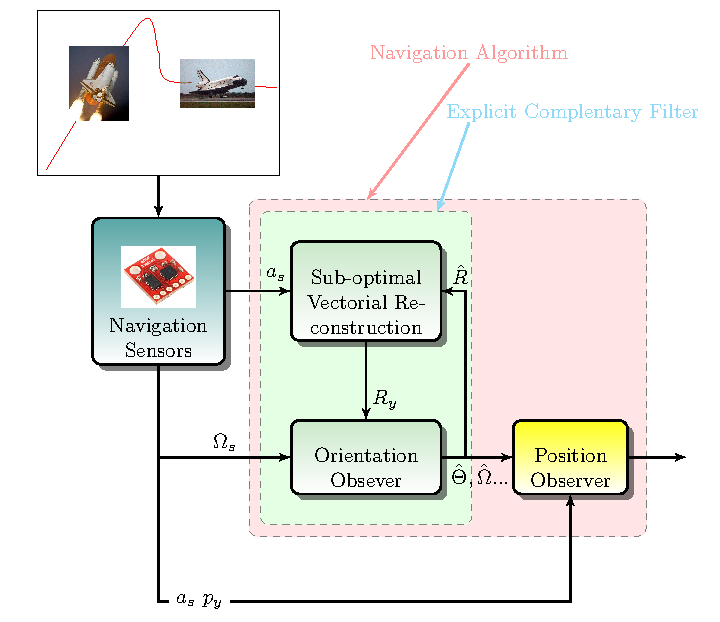
\includegraphics[width=9cm,clip]{ms-algorithm.pdf}
\caption{Simplified scheme of the original navigation algorithm of Mahoni-Scandaroli.}
\scriptsize{The attitude observer utiliza la medición de la velocidad angular $\Omega_s$ \footnote{ Elemento de conjunto de \emph{información sensorial disponible} $S$} y}
\label{solucionMS_fig1}
\end{figure}
The navigation problem lays in the determination of an algorithm that possess the ability to determine the set of variables describing the spatial condition of a rigid body using related set of variables which we term \emph{sensory information} ($S$). In these frame terms the solution as seen through the Mahony-Scandarolli approach derives in the navigation algorithm described in \figurename\ref{solucionMS_fig1} which entails the combination of two nonlinear observers one for attitude and other for position. The measurement of the angular velocity $\Omega_s$ and  the vectorial reconstruction of the rotation matrix $R_y$ are inputs into the attitude observer which determines:
\begin{itemize}
\item $\hat{\Theta}$: Estimation of the Euler angles.
\item $\hat{\Omega}$: Estimation of  the angular velocity in $\marco{B}$, where $\marco{B}$ denotes the body fixed framework.
\item $\tilde{R}$: Rotation matrix error defined as the transformation from $\marco{E}\hookrightarrow\marco{B}$ where $\marco{E}$ denotes the estimation referential framework.
\item $\hat{R}$: The estimation of the rotation matrix that also defines a frame transformation $ \marco{E}\hookrightarrow\marco{A}$ where $\marco{A}$ denotes the inertial frame.
\end{itemize}
Finally, the position complementary filter uses the rest of the variables included in $S$ (the measured acceleration $a_s$ and position $p_y$) and the transformation matrices computed by the previous observer; it determines :
\begin{itemize}
\item $\hat{p}$: Position estimation in $\marco{A}$.
\item $\hat{v}$: Linear velocity estimation in $\marco{A}$.
\end{itemize}
The group of estimation results are concatenated in what we denote \emph{the Navigation Information Estimation } expressed as $X=[\hat{p}~\hat{v}~\hat{\Theta}~\hat{\Omega}]$.\par
%%
Under this scheme, the vectorial reconstruction feeds in the orientation observer with the rotation matrix's reconstruction that depends directly of the weighted sum of the vectorial measurements in the body framework $\marco{B}$ ($V_i$) as well as $\hat{R}$: 
\begin{equation}\label{ReconstruccionVectorial}
R_y=\sum_{i=1}^{n}f(v_i,\hat{R})
\end{equation}
The main disadvantage in the formulation of the complementary filters on SO(3) is the sensibility  to $R_y$ in as much it is involved in the mapping of $\omega_s$ to $\marco{A}$, fot that reason the determination of this matrix play a mayor role. They mention that the optimal solution can be determined in the minimization argument of:
\begin{equation}\label{ProblemaOptimizacion}
R^*=\arg~\min_{R}\left\{\sum_i|V_{0,i}-RV_{m,i}|^2\right\}
\end{equation}
Where the optimal solution  $R^*$ is function of a loss function defined in the sum of euclidean norms of the errors between the vectorial measurements   (R$V_{m,i}$) rotated to $\marco{A}$ with respect to their respective theoretical values ($v_{0,i}$)(Sub-indexes $0$ stays by theoretical and $m$ by measured.). However, Mahony-Scandaroli's algorithm solves $R_y$ through an sub-optimal method depending on $\hat{R}$ so it relies on the Lyapunov statability trajectory.  We assume that the optimal solution of $R_y$ could enhance the general performance of the algorithm.
%%%%%%%%%%%%%%
%%%%%%%%%%%%%%
%%%%%%%%%%%%%%
\section{Optimal reconstruction of Rotation Matrix \label{opt_reconstruction}}
%%
In this section we present the general solution for optimal determination of the rotation matrix that we deem could improve the algorithm's performance. We propose to compute the Rotation Matrix by estimating the inclination of the gravity vector field in $\marco{B}$  with an optimal observer in quaternions  in sense that rotation a rigid body in completely described in terms of the Euler angles $\Theta$ and the angular velocity Intuitively these given states can be determined through the measurement of: the angular speed $\Omega_s$ with a gyroscope and the observation of the attitude $\Theta$ with an accelerometer in the declination of the gravity vector. This approach is possible since the rotation matrix can be expressed in terms of the components of a unitary quaternion \cite{Altmann1986}. Hence, an optimal observer should reduce the deviation measurement of acceleration $a_s$ to its rotated theoretical value $g_0$ in $\marco{A}$.\par
%%%
\begin{figure*}[!t]
\centering
\subfloat[Case I]{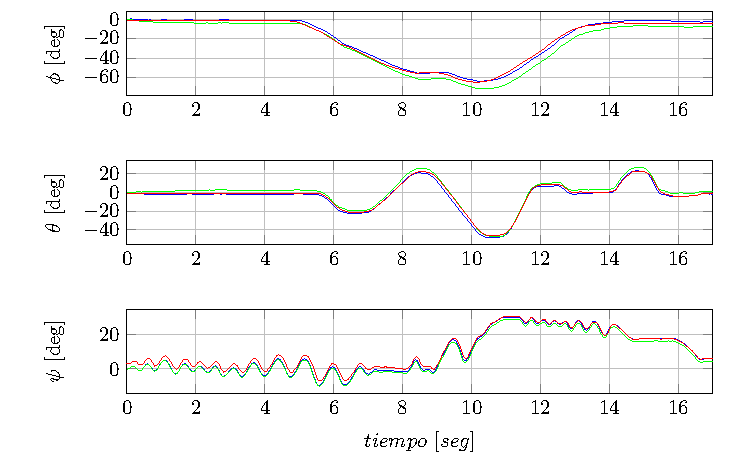
\includegraphics[width=17.3em]{angularTestPaper1.pdf}%
\label{PlotPh1}}
\subfloat[Case II]{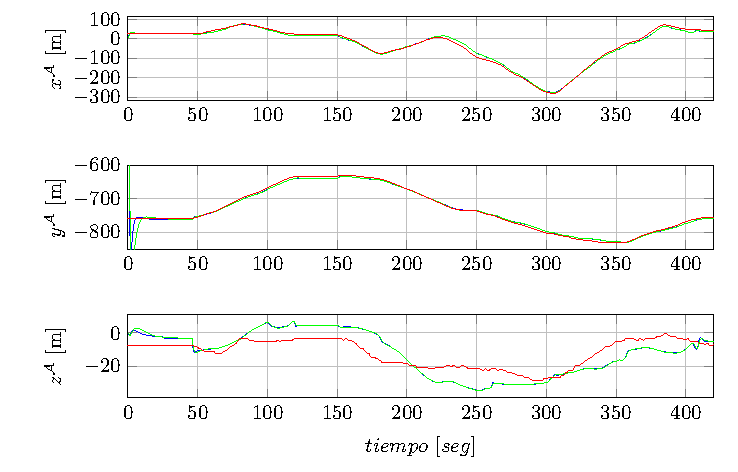
\includegraphics[width=17.3em]{positionTestPaper1.pdf}%
\label{PlotX1}}
\subfloat[Case III]{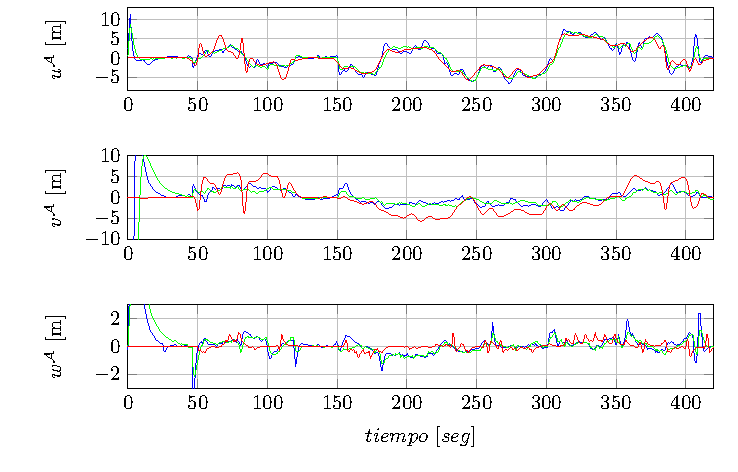
\includegraphics[width=17.3em]{velocityTestPaper1.pdf}%
\label{PlotU1}}
\caption{Simulation results for the network.}
\label{Plots}
\end{figure*}
Therefore, the optimal observer works  to reduce the loss function \eqref{ProblemaOptimizacionAcc} where $R^*$ depends on unitary quaternion $\breve{q}=q_0+q_1i+q_2j+q_3k \in \mathbb{Q} \subset \mathbb{H}$\footnote{$\mathbb{H}$ denotes the Hamiltonian space of quaternion complex numbers $\mathbb{Q}$ is the sub-space of all quaternions with unitary norm.}:
\begin{equation}\label{ProblemaOptimizacionAcc}
R^*(\breve{q})=R\left(q^*=\arg\min_{\breve{q}}\left\{a_s-R^T(\breve{q})g_0\right\}\right)
\end{equation} 
Thereby the solution is given in terms of the optimal unitary quaternion that rotates $g_0$ to $a_s$ which is estimated by $\hat{a}_s$ as follows% \cite{Sola2012}:
\begin{equation}\label{chap2:ModeloMedicion}
\hat{a}_s=\bar{\breve{q}}\otimes\breve{g_0}\otimes\breve{q}=Rg_0=g_0\begin{bmatrix}2(q_1q_3-q_oq_2)\\2(q_2q_3+q_0q_1)\\q_0^2-q_1^2-q_2^2-q_3^2\end{bmatrix}
\end{equation}
This allows us to define that the challenge assumed by the observer is to determine the optimal quaternion at the discrete time $k$ considering the following elements: i)the initial conditions uncertanity for the estimated quaternion $\tilde{q}_0$ y and the measurement deviation $\hat{v}_0$, ii) the model uncertainty $\hat{w}_k$ defined in \eqref{quaMod}\footnote{$f_k$ represents the quaternion kinematics which defined in terms the quaternion product of the unitary quaternion and the angular velocity expressed as pure quaternion.}
iii) the measurement uncertainty, that defines itself as deviation of $\hat{a}_{s,k}$ to $a_{s,k}$ in the dicrete time $k$, that also depends on $\hat{\breve{q}}_{k}$.
\begin{equation}
\label{quaMod}
\hat{\breve{q}}_{k+1}=f_k(\hat{\breve{q}}_k,\Omega_k)+\hat{w}_k
\end{equation}
\begin{equation}
\hat{v}_k=a_{s,k}-\underbrace{\hat{a}_{s,k}}_{\hat{a}_{s,k}=h_k(\hat{\breve{q}}_k)}
\end{equation}
The loss function \eqref{ProblemaOptimizacionAcc} is re-written in terms of two norms in \eqref{loss} where the first combines $\hat{v}_0$ and $\tilde{q}_0$ y the second combines $\hat{w}_k$ and $\hat{v}_k$ within the interval $i\in\{k_0,...,k_f\}$ considering $k_f$ current time. Hereby we propose the solution of the optimization problem finding the next $\hat{\breve{q}}_{k+1}$ in terms of successive corrections of $\hat{w}_k$  that can be obtained from dynamical programming approach \cite{Lewis2012}.\par
\begin{equation}\label{loss}
q^*_k=\arg~\min_{q_k}\left\{norm_0(\tilde{q}_0,\hat{v}_0)+\sum^k_{i=0}norm_1(w_i,v_i)\right\}
\end{equation}
%%%%%%%%%%%%%%%
%%%%%%%%%%%%%%%%
%%%%%%%%%%%%%%%%%
\section{Experimental evaluation Methodology}\label{Metodologia}
In general, the experimental evaluation aims to evaluate reduction of estimation errors by including the optimal observer stage into the original navigation algorithm, that results in what we name the modified navigation algorithm. We studied each case by providing the same input and collecting the results in $\hat{X}_{mdf}$ for the modified algorithm and  $\hat{X}_{mh}$ for the original algorithm these are compared with a reference measurement $X_{real}$ obtained from an external source.
By means of simplicity we reduce the whole experiment into two different study cases: 
\begin{enumerate}[\IEEEsetlabelwidth{8)}]
\item Estimation of Euler angles for independent axis. In this case the rotations were performed for one particular axis at the time, the measurements were simultaneously introduced to both navigation algorithms, and the reference was obtained with a camera that tracked the trajectory of two black marks placed on the box containing the navigation sensors.
\item Estimation of p
osition in a closed trajectory in a urban terrain. In this case the experiments were conducted along long closed tracks in a vehicle were we mount the sensors and a commercial GPS tracker, the former was used as input for the navigation algorithms and the latter as reference signal.
\end{enumerate}
\section{Experimental results}\label{experimentation}
%\begin{figure}
%\begin{center}
%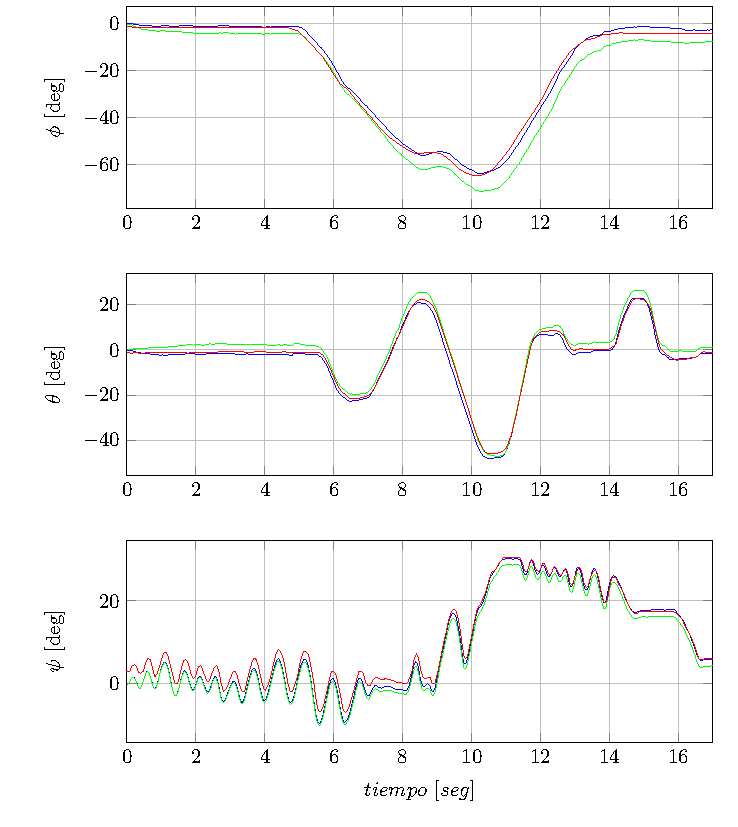
\includegraphics[width=26em]{PlotAngles1.pdf}
%\caption{Prueba comparativa de la estimación de los ángulos de Euler. }
%\label{PlotPh1}
%\scriptsize{Los ángulos de Euler, se denotan en el vector columna $\Theta=[\phi~\theta~\psi]^T$, con $\phi$ para el alabeo, $\theta$ para la rodadura y $\psi$ para el guiñeo. La señal de color azul corresponde a la estimación, la de color verde para el algoritmo original, y de color rojo para la referencia. Las gráficas se ordenan mostrando los resultados de la estimación para los ángulos $\phi$, $\theta$ y $\psi$, ordenados de arriba hacia abajo en el orden en que se los menciona.}
%\end{center}
%\end{figure}
We present a sample of many experiments in Fig.\ref{PlotPh1} for the estimation of the Euler angles, where we observe above the errors moving around within the range $9.04^{\circ}\cdot10^{-3}$ to $10.58^{\circ}$ for the modified approach in contrast to $7.33^{\circ}\cdot10^{-3}$ to $18.97$ for the original  algorithm. In the second case angles rates are within $\pm45[º/s]$ range, and also for this case we observe that the modified algorithm catches the reference nearer that original  after the 13 seconds. Finally, for the third case we experiment with abrupt changes of direction, in addition the gravity vector is parallel to rotating axis what difficulties the vectorial reconstruction. In this graph the error is progressively reduced by the modified algorithm in contrast to the original algorithm which seems to remain in $1.5º$ along at least for the time window that encloses this particular essay.\par
%%
%\begin{figure}
%\begin{center}
%\includegraphics[width=25em]
%{PlotPosition1.pdf}
%\caption{Resultados de la estimación de la posición.}
%\scriptsize{Resultados de la estimación de con datos simulados. Resultados típicos del repetidos intentos. En todas las gráficas, los resultados de la estimación del algoritmo Original son representados en la línea de color verde, para la estimación del algoritmo modificado de color azul, y para la señal de referencia en una línea de color rojo.
%}
%\label{PlotPh1PlotX1}
%\end{center}
%\end{figure}
%%
%%
The results in the case of the linear movement are presented in Fig.\ref{PlotX1} for position and in Fig.\ref{PlotU1} for velocity. We observed that the errors varies around before the transitory stage $2[m]$ y $10[m]$ in the axis $x$ and $y$, further in the horizontal axis tend to be bigger above $20[m]$ which typically are bigger. Regarding the linear velocity some spikes in both algorithms but they seem to follow the reference.\par
%\begin{figure}
%\begin{center}
%\includegraphics[width=25em]
%{PlotVelocity1.pdf}
%\caption{Velocidad lineal en el eje X.}
%\scriptsize{Resultados de la estimación de con datos simulados. Resultados típicos del repetidos intentos.}
%\label{PlotPh1PlotX1PlotU1}
%\end{center}
%\end{figure}
%%%
\section{Comparative Analysis}
In order to compare the results, we used two different metrics: the mean absolute percentage error (MAPE) for each variable's performance , and the relative difference in percentage (PRD) to compare results between algorithms. The results are arrange in the table \ref{resultados_tb1} where we identify a better performance for the modified algorithm compared to the original version. The mean of all PRDs (MPRD) reinforces this statement placing itself in 40.92\%, namely we obtained an average 42.92\% better performance by including a optimal pre-computing of $R^*$ compared with the original approach. In addition, notice that  best relations within the MAPE pairs rest on $y$ i.e. $1.22[m]$ MAPE and the pitch and roll angles i.e. $2.39º$ and $1.73º$ MAPE respectively.\par
\begin{table}[!t]
\caption{Modified and original algorithms comparative table.}
\label{resultados_tb1}
\begin{center}\scriptsize
\begin{tabular}{|p{0.7in}|p{0.6in}|p{0.6in}|p{0.7in}|} \hline
\textbf{Estimation}&\textbf{MAPE modified}&\textbf{MAPE original}&\textbf{PRD modified vs. original.} \\ \hline
%--------------------------------------------------------------------->
X position ($x$) &5.8862[m]&5.9427[m]&0.9596\%\\ \hline
Y  position ($y$) &3.5445[m]&4.7739[m]&34.6828\%\\ \hline
Z  position ($z$)&6.1698[m]&6.3369[m]&2.7080\%\\ \hline
X-velocity ($v_x$) &0.8214[m/s]&0.7871[m/s]&{-12.1305\%}\\ \hline
Y-velocity ($v_y)$&3.1564[m/s]&3.3291[m/s]&5.4710\%\\ \hline
Z-velocity ($v_z$)&0.4445[m/s]&0.5697[m/s]&28.1664\%\\ \hline
Pitching ($\phi$ )&1.3579~$[^{\circ}]$&3.7560~$[^{\circ}]$&177.97\%\\ \hline
Rolling ($\theta$ )&1.4635~$[^{\circ}]$&2.801~$[^{\circ}]$&91.394\%\\ \hline
Yawing ($\psi$ )&1.3268~$[^{\circ}]$&2.1855~$[^{\circ}]$&44.53\%\\ \hline
\end{tabular}
\end{center}
\end{table}
We also perform a processing time comparison where we measure the times to process samples sets of $2957$ points within a $49.4311 [s]$ time window. We obtained and average time for ten essays of $1.0158[ms]$ for the modified algorithm in contrast to $0.7954 [ms]$ for the original algorithm, i.e a MPRD:
\begin{equation}
MPRD_{\texttt{processing time}}=-21.6933\%
\end{equation}
This expression points out that the original algorithm uses $21.6933\%$ less time than the modified.



% An example of a floating figure using the graphicx package.
% Note that \label must occur AFTER (or within) \caption.
% For figures, \caption should occur after the \includegraphics.
% Note that IEEEtran v1.7 and later has special internal code that
% is designed to preserve the operation of \label within \caption
% even when the captionsoff option is in effect. However, because
% of issues like this, it may be the safest practice to put all your
% \label just after \caption rather than within \caption{}.
%
% Reminder: the "draftcls" or "draftclsnofoot", not "draft", class
% option should be used if it is desired that the figures are to be
% displayed while in draft mode.
%
%\begin{figure}[!t]
%\centering
%\includegraphics[width=2.5in]{myfigure}
% where an .eps filename suffix will be assumed under latex, 
% and a .pdf suffix will be assumed for pdflatex; or what has been declared
% via \DeclareGraphicsExtensions.
%\caption{Simulation results for the network.}
%\label{fig_sim}
%\end{figure}

% Note that the IEEE typically puts floats only at the top, even when this
% results in a large percentage of a column being occupied by floats.


% An example of a double column floating figure using two subfigures.
% (The subfig.sty package must be loaded for this to work.)
% The subfigure \label commands are set within each subfloat command,
% and the \label for the overall figure must come after \caption.
% \hfil is used as a separator to get equal spacing.
% Watch out that the combined width of all the subfigures on a 
% line do not exceed the text width or a line break will occur.
%
%\begin{figure*}[!h]
%\centering
%\subfloat[Case I]{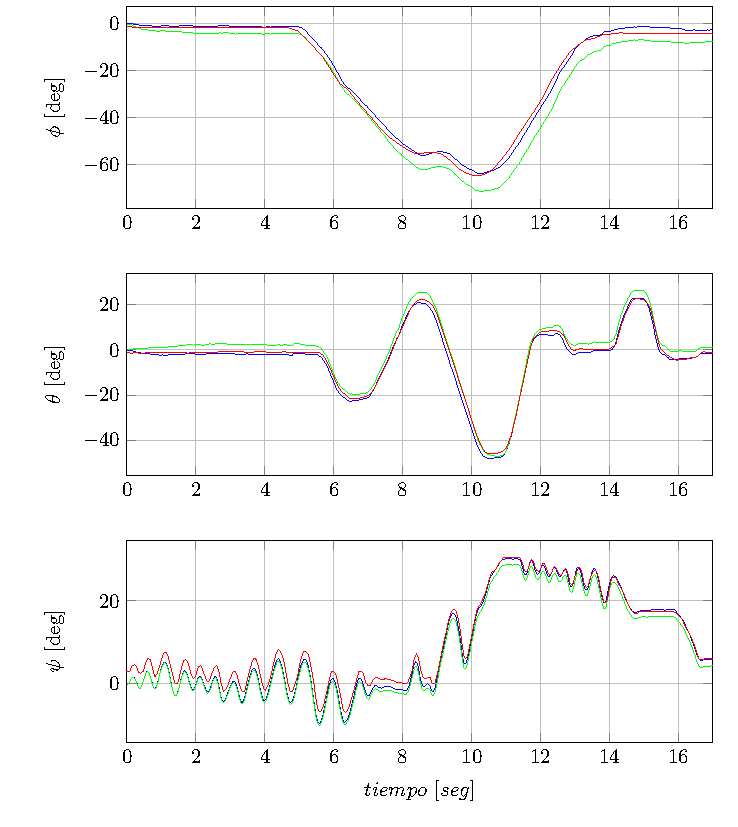
\includegraphics[width=2.5in]{PlotAngles1.pdf}%
%\label{fig_first_case}}
%\subfloat[Case II]{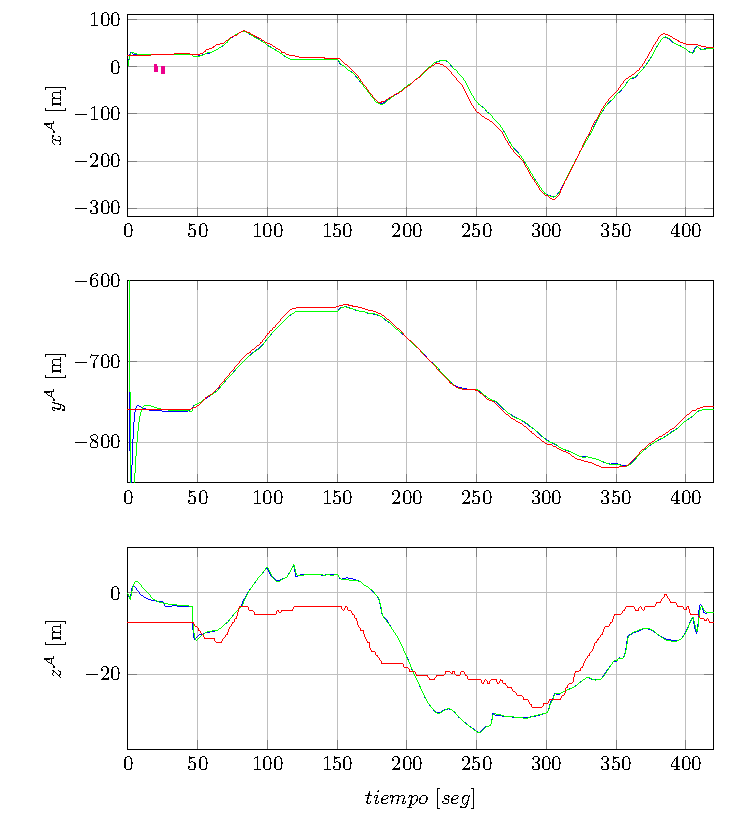
\includegraphics[width=2.5in]{PlotPosition1.pdf}%
%\label{fig_second_case}}
%\subfloat[Case III]{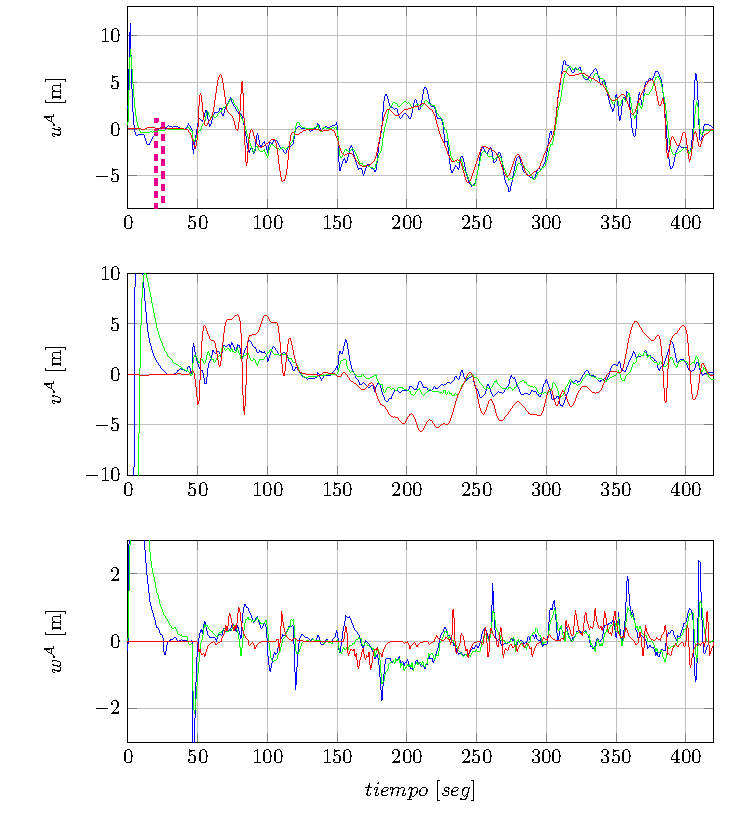
\includegraphics[width=2.5in]{PlotVelocity1.pdf}%
%\label{fig_second_case}}
%\caption{Simulation results for the network.}
%\label{fig_sim}
%\end{figure*}
%
% Note that often IEEE papers with subfigures do not employ subfigure
% captions (using the optional argument to \subfloat[]), but instead will
% reference/describe all of them (a), (b), etc., within the main caption.
% Be aware that for subfig.sty to generate the (a), (b), etc., subfigure
% labels, the optional argument to \subfloat must be present. If a
% subcaption is not desired, just leave its contents blank,
% e.g., \subfloat[].


% An example of a floating table. Note that, for IEEE style tables, the
% \caption command should come BEFORE the table and, given that table
% captions serve much like titles, are usually capitalized except for words
% such as a, an, and, as, at, but, by, for, in, nor, of, on, or, the, to
% and up, which are usually not capitalized unless they are the first or
% last word of the caption. Table text will default to \footnotesize as
% the IEEE normally uses this smaller font for tables.
% The \label must come after \caption as always.
%
%\begin{table}[!t]
%% increase table row spacing, adjust to taste
%\renewcommand{\arraystretch}{1.3}
% if using array.sty, it might be a good idea to tweak the value of
% \extrarowheight as needed to properly center the text within the cells
%\caption{An Example of a Table}
%\label{table_example}
%\centering
%% Some packages, such as MDW tools, offer better commands for making tables
%% than the plain LaTeX2e tabular which is used here.
%\begin{tabular}{|c||c|}
%\hline
%One & Two\\
%\hline
%Three & Four\\
%\hline
%\end{tabular}
%\end{table}


% Note that the IEEE does not put floats in the very first column
% - or typically anywhere on the first page for that matter. Also,
% in-text middle ("here") positioning is typically not used, but it
% is allowed and encouraged for Computer Society conferences (but
% not Computer Society journals). Most IEEE journals/conferences use
% top floats exclusively. 
% Note that, LaTeX2e, unlike IEEE journals/conferences, places
% footnotes above bottom floats. This can be corrected via the
% \fnbelowfloat command of the stfloats package.




\section{Conclusion}
In this work we proposed a observer architecture composed by non-linear complementary filters on the $SO(3)$ and an optimal observer of the rotation matrix, this considers the signals coming from an inertial measurement unit (IMU)  and a GPS receptor as inputs. In addition, we carried out an experimental exploration of the properties of both algorithms in the same conditions in order to obtain comparable information. Based on the experimental results we deem  important to point out that the navigation algorithms including an optimal estimation of the rotation matrix does better in estimation than the algorithm computing the rotation matrix with sub-optimal vectorial reconstruction, however such modification involves a considerable increment of complexity. 
% use section* for acknowledgment
\section*{Acknowledgment}
The author would like to thank to the University faculties for their support and collaboration. 
% trigger a \newpage just before the given reference
% number - used to balance the columns on the last page
% adjust value as needed - may need to be readjusted if
% the document is modified later
%\IEEEtriggeratref{8}
% The "triggered" command can be changed if desired:
%\IEEEtriggercmd{\enlargethispage{-5in}}

% references section

% can use a bibliography generated by BibTeX as a .bbl file
% BibTeX documentation can be easily obtained at:
% http://mirror.ctan.org/biblio/bibtex/contrib/doc/
% The IEEEtran BibTeX style support page is at:
% http://www.michaelshell.org/tex/ieeetran/bibtex/
%\bibliographystyle{IEEEtran}
% argument is your BibTeX string definitions and bibliography database(s)
%\bibliography{IEEEabrv,BiblioTh7}
%
% <OR> manually copy in the resultant .bbl file
% set second argument of \begin to the number of references
% (used to reserve space for the reference number labels box)
\bibliographystyle{IEEEtran}
% argument is your BibTeX string definitions and bibliography database(s)
\bibliography{IEEEabrv,BiblioTh7}



%\begin{thebibliography}{1}
%\bibitem{Kalman1960}
%H.~Kopka and P.~W. Daly, \emph{A Guide to \LaTeX}, 3rd~ed.\hskip 1em plus
%  0.5em minus 0.4em\relax Harlow, England: Addison-Wesley, 1999.
%\bibitem{Lukyanov1996}
%H.~Kopka and P.~W. Daly, \emph{A Guide to \LaTeX}, 3rd~ed.\hskip 1em plus
%  0.5em minus 0.4em\relax Harlow, England: Addison-Wesley, 1999.
%\bibitem{Nicosia1996}
%H.~Kopka and P.~W. Daly, \emph{A Guide to \LaTeX}, 3rd~ed.\hskip 1em plus
%  0.5em minus 0.4em\relax Harlow, England: Addison-Wesley, 1999.
%\bibitem{Algrain1997}
%H.~Kopka and P.~W. Daly, \emph{A Guide to \LaTeX}, 3rd~ed.\hskip 1em plus
%  0.5em minus 0.4em\relax Harlow, England: Addison-Wesley, 1999.
%\bibitem{Vasconcelos2008}
%H.~Kopka and P.~W. Daly, \emph{A Guide to \LaTeX}, 3rd~ed.\hskip 1em plus
%  0.5em minus 0.4em\relax Harlow, England: Addison-Wesley, 1999.
%\bibitem{Scandaro2011}
%H.~Kopka and P.~W. Daly, \emph{A Guide to \LaTeX}, 3rd~ed.\hskip 1em plus
%  0.5em minus 0.4em\relax Harlow, England: Addison-Wesley, 1999.
%\bibitem{Schmidt1962}
%H.~Kopka and P.~W. Daly, \emph{A Guide to \LaTeX}, 3rd~ed.\hskip 1em plus
%  0.5em minus 0.4em\relax Harlow, England: Addison-Wesley, 1999.
%\bibitem{Grewal 2010}
%Mohinder Grewal, Angus Andrews. (2010) Applications of Kalman Filtering in Aerospace 1960 to the Present [Historical Perspectives. IEEE Control Systems Magazine 30:3, 69-78
%Online publication date: 1-Jun-2010. Read More: http://arc.aiaa.org/doi/abs/10.2514/3.19713
%\bibitem{Bistrovs2012}
%H.~Kopka and P.~W. Daly, \emph{A Guide to \LaTeX}, 3rd~ed.\hskip 1em plus
%  0.5em minus 0.4em\relax Harlow, England: Addison-Wesley, 1999.
%\bibitem{Gandhi2007}
%H.~Kopka and P.~W. Daly, \emph{A Guide to \LaTeX}, 3rd~ed.\hskip 1em plus
%  0.5em minus 0.4em\relax Harlow, England: Addison-Wesley, 1999.
%\bibitem{Sabatini2006}
%H.~Kopka and P.~W. Daly, \emph{A Guide to \LaTeX}, 3rd~ed.\hskip 1em plus
%  0.5em minus 0.4em\relax Harlow, England: Addison-Wesley, 1999.
%\bibitem{Luenberger 1966}
%Luenberger D G. Observers for multivariable systems. IEEE
%Trans. Automat. Contr. AC-11:190-7, 1966. [Dept. Electrical
%Engineering, Stanford Univ., Stanford, CA]
%\bibitem{Kou1973}
%\bibitem{Thau1973}
%\bibitem{Vik2001}
%\bibitem{Thienel2003}
%\bibitem{Hua2009}
%\bibitem{Bonabel2008}
%\bibitem{Bonabel2005}
%\bibitem{Mahony2008}
%\end{thebibliography}




% that's all folks
\end{document}


